\chapter{Prototypische Umsetzung\label{chap5:Fuenftes-Kapitel}}

Im folgenden Kapitel wird die Umsetzung des Prototypen vorgestellt. Neben einer Einführung in den Funktionsumfang des Prototypen, wird das Gesamtkonzept aus \autoref{sec4.3:Unterpunkt-3} in verschiedene Komponenten unterteilt.

% ToDo more Text

\section{Funktionsumfang\label{sec5.1:Unterpunkt-1}}

Der Umfang des Prototypen soll eine Bibliothek darstellen, in welcher ein Benutzer die Möglichkeit besitzt Bücher anzulegen und zu verwalten. Hierfür werden die allgemeinen CRUD-Operationen zur Verfügung gestellt. Der Benutzer hat demnach die Möglichkeit neue Bücher dem Bestand hinzuzufügen (Create), sich den aktuellen Bestand anzeigen zu lassen (Read), bestehende Bücher zu ändern (Update) oder Bücher aus dem Bestand zu entfernen.

In \autoref{fig:UserInterface} ist die Benutzerschnittstelle abgebildet.

\begin{figure}[H]
    \centering
    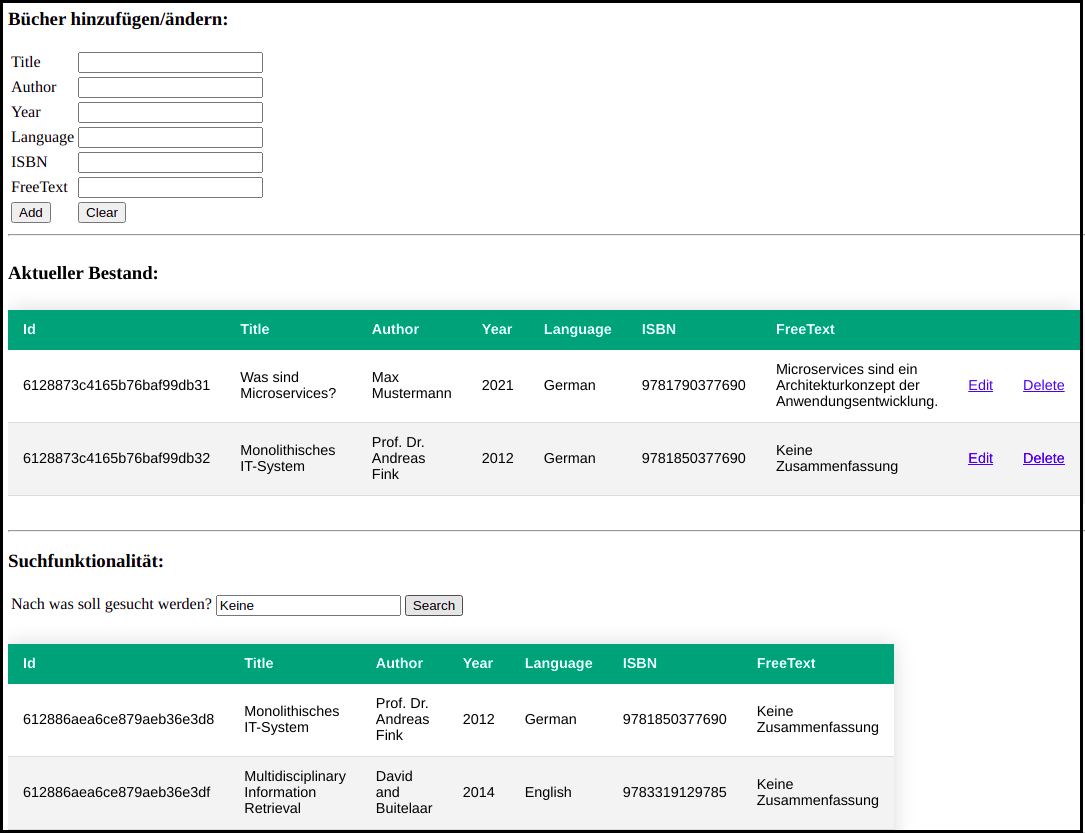
\includegraphics[width=0.9\linewidth]{images/UserInterface.png}
    \caption{Benutzeransicht der prototypischen Umsetzung}
    \label{fig:UserInterface}
\end{figure}

Zu unterteilen ist die Ansicht in drei Bereiche \glqq Bücher hinzufügen/ändern\grqq{}, \glqq Aktueller Bestand\grqq{} und \glqq Suchfunktionalität\grqq{}.

Im oberen Bereich haben die Benutzer die Möglichkeit neue Bücher dem Bestand hinzuzufügen. Durch Betätigung des Buttons \glqq Add\grqq{} werden die Informationen aus den darüberliegenden Feldern als neues Objekt in der Datenhaltung abgespeichert. Zusätzlich dient der obere Bereich der Bearbeitung bestehender Bücher. Hierfür wird im darunterliegenden Datenbestand das jeweilige Buch durch den Button \glqq Edit\grqq{} ausgewählt und die enthaltenen Informationen können anschließend bearbeitet und gespeichert werden. Durch Betätigung des Buttons \glqq Clear\grqq{} werden die Text- und Zahlenfelder geleert.

Der aktuelle Bestand der Bücher in der Datenhaltung, wird in einer Tabelle wiedergegeben. Angezeigt werden neben einer eindeutigen ID auch die Informationen Titel, Autor, Veröffentlichungsjahr, Sprache, ISBN und Zusammenfassung. Jede Reihe der Tabelle repräsentiert ein Buch-Objekt aus der Datenhaltung und kann jeweils durch den Button \glqq Edit\grqq{} bearbeitet oder durch den Button \glqq Delete\grqq{} entfernt werden.

Im unteren Bereich der Benutzerschnittstelle findet sich die Suchfunktionalität. Der Benutzer hat hierbei die Möglichkeit in das Textfeld eine beliebige Suchphrase einzugeben. Durch Betätigung des Buttons \glqq Search\grqq{} wird die Suchphrase an die Search Engine geschickt und die empfangenen Suchtreffer werden in der darunterliegenden Tabelle angezeigt.

Neben der reinen Eingabe einer Suchphrase könne auch Wildcards für die Suche verwendet werden. Unterstützt werden von Elasticsearch unter anderem die Wildcards \glqq ?\grqq{} und \glqq *\grqq{}. \glqq ?\grqq{} ersetzt dabei genau ein beliebiges Symbol, während durch \glqq *\grqq{} keine oder mehrere Symbol ersetzt werden.

Zusätzlich zu den Wildcards können auch die Attribute angegeben werden, über welche die Suche ausgeführt werden soll. Standardmäßig wird bei der Suche über alle vorhandenen Attribute gesucht. So ist es durch die Eingabe von \glqq status:active\grqq{} möglich, nach dem Begriff \glqq active\grqq{} in dem Attribut \glqq status\grqq{} zu suchen.

\section{Komponenten\label{sec5.2:Unterpunkt-2}}

Unterteilt werden kann das Gesamtkonzept aus \autoref{sec4.3:Unterpunkt-3} in die drei Bereiche \glqq Book Service\grqq{}, \glqq CDC-Datenpipeline\grqq{} und \glqq Search Engine\grqq{}.

\subsection{Book Service\label{sec5.2.1:Unterunterpunkt-1}}

Für das Anlegen und Verwalten der Bücher in der Bibliothek ist der Book Service zuständig. Umgesetzt wurde der Service mit der Programmiersprache Golang und der Datenbank MongoDB.

Neben der Bereitstellung einer REST API für das Anlegen und Verwalten von Büchern übernimmt der Book Service zusätzlich das Hosten der Website. Hierfür werden über eine zusätzliche REST API die Webinhalte für den Client zur Verfügung gestellt. Die interne Weiterleitung der eingehenden Anfragen übernimmt ein Go-Webserver. Dieser leitet eingehende Anfragen anhand von vordefinierten Routing-Pfaden an die Anwendung weiter.

\autoref{fig:BookService} zeigt einen Ausschnitt des Book Services aus dem Gesamtkonzept.

\begin{figure}[H]
    \centering
    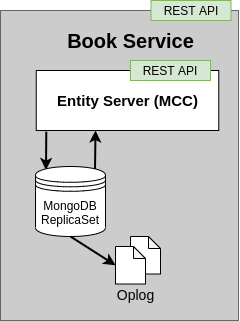
\includegraphics[width=0.3\linewidth]{images/BookService.png}
    \caption{Teil des Gesamtkonzeptes: Book Service}
    \label{fig:BookService}
\end{figure}

Für die direkte Kommunikation mit der Datenhaltung wird das Software-Modul \glqq Entity Server\grqq{} von MCC verwendet. Für den Prototypen abstrahiert der Entity-Server die Kommunikation mit der Datenbank MongoDB. Neben der Abstraktion der Datenbank-Kommunikation bietet der Entity-Server die Möglichkeit, Entitäten über eine REST API in der Datenhaltung anzulegen und zu verwalten.

Für die spätere Ankopplung an die CDC-Software Debezium muss die Datenbank MongoDB entweder als \glqq Replica Set\grqq{} oder \glqq Shared Cluster\grqq{} gestartet werden. Dies ist notwendig, da Debezium das Transaktionsprotokoll \glqq OpLog\grqq{} für die Erkennung der Datenänderungen benötigt. MongoDB verwendet dieses Transaktionsprotokoll für die Synchronisierung er einzelnen MongoDB-Instanzen innerhalb eines Replica Sets oder einem Shared Cluster.

Die REST API des Book Service wird unter dem Port 8080 veröffentlicht und beinhaltet die folgenden Schnittstellenendpunkte:

\begin{itemize}
    \item GET - \glqq /book\grqq{} => Gebe alle Bücher zurück
    \item POST - \glqq /book\grqq{} => Füge ein neues Buch hinzu
    \item PUT - \glqq /book\grqq{} => Aktualisiere ein bestimmtes Buch
    \item DELETE - \glqq /book\grqq{} => Entferne ein bestimmtes Buch
    \item GET - \glqq /search/{searchString}\grqq{} => Gebe alle Ergebnisse für den Parameter zurück
    \item GET - \glqq /MCC-Bibliothek\grqq{} => Gebe dem Client die Webinhalte (HTML, CSS, JavaScript)
\end{itemize}

\subsection{CDC-Datenpipeline\label{sec5.2.2:Unterunterpunkt-2}}

Um die Datenaktualisierung zwischen den Datenhaltungsschichten und der Search Engine zu ermöglichen, wird für den Prototypen die CDC-Aktualisierung verwendet. Die gesamte Datenpipeline besteht aus dem Message Broker \glqq Apache Kafka\grqq{} und den Kafka-Konnektoren \glqq Debezium-MongoDB-Connector\grqq{} und \glqq Elasticsearch-Sink-Connector\grqq{}.

\autoref{fig:CDC-Pipeline} zeigt einen Ausschnitt der CDC-Datenpipeline aus dem Gesamtkonzept.

\begin{figure}[H]
    \centering
    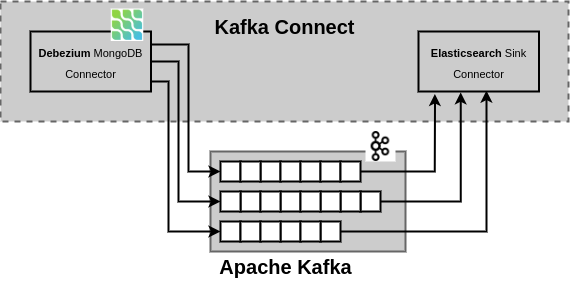
\includegraphics[width=0.7\linewidth]{images/CDC-Pipeline.png}
    \caption{Teil des Gesamtkonzeptes: CDC-Datenpipeline}
    \label{fig:CDC-Pipeline}
\end{figure}

Gestartet werden die Komponenten der Datenpipeline in Docker Containern. Hierzu wird ein Kafka und ein Kafka-Connect Container gestartet.

Kafka-Connect dient hierbei der Anbindung von Drittsystemen an Kafka. Innerhalb des Prototypen sind Anbindungen an die Datenbanken MongoDB und Elasticsearch notwendig. Hierfür werden die passenden Konnektoren über Kafka-Connect aktiviert. Konnektoren können dabei in zwei Kategorien unterteilt werden.

\begin{description}
    \item[Source Konnektoren:]\hfill \\
    Die Source Konnektoren sind für die Nachrichtenweiterleitung aus den verschiedenen Datenquellen hin zu Kafka zuständig. Als Producer schicken diese Konnektoren Informationen an Kafka-Topics.
    
    \item[Sink Konnektoren:]\hfill \\ 
    Für die Weiterleitung der Informationen aus den Kafka-Topics zu Drittsystemen sind die Sink Konnektoren zuständig. Sie fungieren hierbei als Consumer an den jeweiligen Kafka-Topics.

\end{description}

Die Nachrichten innerhalb des Prototypen werden im Datenformat JSON weitergeleitet. Um die Kompatibilität der Konnektoren untereinander zu gewährleisten ist eine Transformation der Nachrichten notwendig. Aus diesem Grund wurde beim Prototypen eine Transformation der JSON-Nachrichten beim Source Konnektor durchgeführt.

%\begin{lstlisting}[language=json,firstnumber=1]
%{
%  "name": "mongo",
%  "config": {
%      "connector.class": "io.debezium.connector.mongodb.MongoDbConnector",
%      "mongodb.hosts": "mongo:27017",
%      "mongodb.name": "mongoconnector",
%      "mongodb.user": "user",
%      "mongodb.password": "pwd",
%      "MongoDB.authsource": "admin",
%      "value.converter": "org.apache.kafka.connect.json.JsonConverter",
%      "value.converter.schemas.enable": "false",
%      "transforms": "unwrap",
%      "transforms.unwrap.type": "io.debezium.connector.mongodb.transforms.ExtractNewDocumentState",
%      "transforms.unwrap.drop.tombstones": "false",
%      "transforms.unwrap.delete.handling.mode": "drop",
%      "transforms.unwrap.operation.header": "true"
%  }
%}
%\end{lstlisting}

%\begin{lstlisting}[language=json,firstnumber=1]
%{
%    "name": "elasticsearch",
%    "config": {
%        "connector.class": "io.confluent.connect.elasticsearch.ElasticsearchSinkConnector",
%        "connection.url": "http://elasticsearch:9200",
%        "tasks.max": "1",
%        "topics": "mongoconnector.mcc-bibliothek.books",
%        "type.name": "_doc",
%        "value.converter": "org.apache.kafka.connect.json.JsonConverter",
%        "value.converter.schemas.enable": "false",
%        "schema.ignore": "true",
%        "behavior.on.null.values": "IGNORE",
%        "transforms": "InsertKey, ExtractId",
%        "transforms.InsertKey.type": "org.apache.kafka.connect.transforms.ValueToKey",
%        "transforms.InsertKey.fields": "id",
%        "transforms.ExtractId.type": "org.apache.kafka.connect.transforms.ExtractField$Key",
%        "transforms.ExtractId.field": "id"
%    }
%}
%\end{lstlisting}

\subsection{Search Service\label{sec5.2.3:Unterunterpunkt-3}}

Ein weiterer Bestandteil des Prototypen ist der Search Service, welcher die eigentliche Search Engine beinhaltet. Aufgrund der Kompatibilität mit dem Message Broker Kafka und dem Vorliegen eines Kafka-Konnektoren, wurde sich für die Search Engine Elasticsearch entschieden.

\autoref{fig:SearchService} zeigt einen Ausschnitt des Search Services aus dem Gesamtkonzept.

\begin{figure}[H]
    \centering
    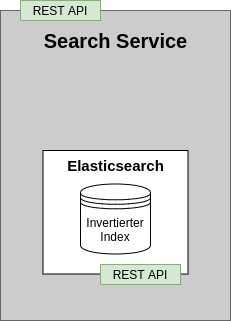
\includegraphics[width=0.3\linewidth]{images/SearchService.png}
    \caption{Teil des Gesamtkonzeptes: Search Service}
    \label{fig:SearchService}
\end{figure}

Durch die Verwendung der REST API, welche von Elasticsearch zur Verfügung gestellt wird, ist es möglich neue Datenänderungen für die Indexierung zu übergeben. Zudem wird eine Schnittstelle für das Stellen einer Suchanfrage zur Verfügung gestellt. Die interne Erstellung und Verwaltung des invertierten Indexes wird hierbei komplett von Elasticsearch übernommen.

Für die Umsetzung des Prototypen wurden die Standard-Konfigurationen von Elasticsearch verwendet. Die zahlreichen Konfigurationsmöglichkeiten für die Indexierung und für die verschiedenen Transformationsschritte, gilt es in weiterführenden Untersuchungen zu erläutern.